\documentclass{beamer}
\usepackage[utf8]{inputenc}

\hypersetup{
    colorlinks,%
    citecolor=blue,%
    filecolor=blue,%
    linkcolor=blue,%
    urlcolor=blue 
    %urlcolor=mygreylink     % can put red here to better visualize the links
}

\author[Sowmya Vajjala]{Instructor: Sowmya Vajjala}

\title[LING 520]{LING 520: Computational Analysis of English}
\subtitle{Semester: FALL '16}

\date{13 September 2016}

\institute{Iowa State University, USA}
%%%%%%%%%%%%%%%%%%%%%%%%%%%

\begin{document}

\begin{frame}\titlepage
\end{frame}

%Assignment 1 discussion: 15min
%Questions about tokenizing and sentence splitting: assuming we dont have capitalization, how will you write a sentence splitter?
%normalizatio: motivation.
%Types of normalization: stop word removal, rare word removal - where are these used
%lowercasing: when is it good, when is it not good.
%normalizing contractions, repetitions (looooove for love etc) etc
%spelling normalization
%spelling correction
%Spelling correction, Normalization algos etc: 30 min
%Assignment 2 description: 10 min
%spelling corrector Norvig stuff?
%Spelling correction API
%Problem Set 2: Practice in class.

\begin{frame}
\frametitle{Class outline}
\begin{itemize}
\item Assignment 1 discussion
\item Revision of tokenization and sentence splitting
\item Assignment 2 description
\item Text normalization and spelling correction: overview
\item Problem Set 2 practice in Class
\end{itemize}
\end{frame}

\begin{frame}
\frametitle{Assignment 1 Discussion}
I need volunteers to discuss their solutions to Assignment 1.
\end{frame}%10min

\begin{frame}
\frametitle{Tokenization and Sentence Splitting: Revision}
\begin{itemize}
\item Did you write your own tokenizer, sentence splitter, and test how they are doing? 
\item What were the patterns they missed? \pause
\item Did you explore tokenizing and sentence splitting options in NLTK?
\item How do they work? Did you find cases where they fail? 
\pause \item What is the difference between WordPunktTokenizer and PunktWordTokenizer? \pause
\item Did anyone check out NLTK's tokenizing and sentence splitting options for a non-English language?
\end{itemize}
\end{frame}

\begin{frame}
\frametitle{Assignment 2 Description}
File on Blackboard (3 Questions, 5 marks for each). \\ Deadline: 27 September. 
\end{frame} %10min

\begin{frame}
\frametitle{Why/When are these different pre-processing tasks done?}
\begin{enumerate}
\item lower casing \pause
\item tokenization, sentence splitting \pause
\item removing most frequent, or most rare words \pause 
\item stemming, lemmatization \pause
\item text normalization: substituting contractions, abbreviations, spelling normalization and correction etc. \pause
\end{enumerate}
\end{frame}

%date formats, abbreviations etc: useful in speech recognition kind of things.
%lowercasing, removing most freq, most rare: useful in bag of words approaches
%spelling normalization: useful in IR, to retrieve different spellings of same word in search results. 

\begin{frame}
\frametitle{How do you do these tasks?}
\begin{enumerate}
\item removing most frequent or most rare words \pause
\item If am not talking about English, think about any other language you know, and tell if the task is as simple. \pause
\item substituting contractions \pause
\item substituting abbreviations \pause
\item converting all dates into one standard form \pause
\item stemming \pause
\item lemmatization
\end{enumerate}
\end{frame}

\begin{frame}
\frametitle{Text Normalization}
\begin{itemize}
\item Normalization refers to all forms of pre-processing that tries to bring text representations into some standard form (lower casing, substituting abbreviations etc.)
\item Reason: makes comparison between documents/words easier
 \item normalization may look like a simple, straight forward task which can be done with regular expressions and string substitutions. 
\item However, there are several design issues. Here is a graduate level course on text normalization: \url{http://www.csee.ogi.edu/~sproatr/Courses/TextNorm/}
\item Today's class: two forms of spelling normalization - soundex, edit distance.
\end{itemize}
\end{frame}

\begin{frame}
\frametitle{Name normalization: Soundex Algorithm}
\begin{itemize}
\item The purpose of name normalization methods is to capture different spelling variations of proper names.
\item Soundex is one such method, which is a phonetic algorithm for English names. The goal is to group similar sounding names together. This is mainly useful in information retrieval from databases etc.
\item Very first algorithm is almost a century old now!
\item Simple rules, and straight forward mapping. 
\item Any surname gets converted to a code of a single character and three digits seperated by hyphen.
\end{itemize}
\end{frame}

\begin{frame}
\frametitle{Soundex coding rules}
\url{http://www.archives.gov/research/census/soundex.html}
\\(Use this to answer a question in Assignment 2)
\end{frame}

\begin{frame}
\frametitle{Spelling normalization}
\framesubtitle{The idea of "distance between words"}
\begin{itemize}
\item "distance between words" refer to some way of quantifying how much two words are seperated from each other orthographically.
\item This is useful in applications such as information retrieval (for capturing spelling variations), spelling suggestions (suggesting the closest possible alternative to an unknown word).
\item Several measures of orthographic distance exist: \url{https://en.wikipedia.org/wiki/Category:String_similarity_measures}
\item I will discuss one: Minimum edit distance, and introduce the concept of "dynamic programming" through that on thursday
\end{itemize}
\end{frame}

\begin{frame}
\frametitle{Minimum edit Distance: Introduction}
\begin{itemize}
\item Idea: minimum number of edits required to transform one word into another.
\item What are edits: insertions, deletions, substitutions
\item From Creep to Crap, there is one deletion (remove one e) and one substitution (second e to a)
\item From Sleep to slept, there are: one deletion (delete second e), one insertion (insert t) \pause
\item Alternative: 2 substitutions. Substitutions in edit distance metrics have more penalty though. 
\end{itemize}
\end{frame}

\begin{frame}
\frametitle{Other measures of Similarity between words}
\begin{itemize}
\item distributional similarity: words that are used in similar contexts are perhaps related to each other
\item other form of semantic similarity: computed based on the presence of large lexico-semantic resources like wordnet.
\item \url{http://wordnet.princeton.edu}
\item Chapter 2.5 in NLTK book has an overview of some such measures available in NLTK.
\item Useful for some NLP problems like word sense disambiguation.
\end{itemize}
\end{frame}

\begin{frame}
\frametitle{Next Class}
\begin{itemize}
\item Continuation of spell check/correction discussion.
%\item Introduction to Morphological Analysis; Stemming and Lemmatization overview
\item Optional to do: Read "How to write a spelling corrector" by Peter Norvig (\url{http://norvig.com/spell-correct.html})
\item One announcement: On thursday, our class will take place in Ross 420. 
\end{itemize}
\end{frame}

\begin{frame}
\frametitle{Practice exercises}
\begin{enumerate}
\item Figure out whether NLTK has a distance metric such as levenshtein or other such orthographic distances, and learn how to use one such measure to get distance between words.
\item Check for any python based spell checking libraries. If you do not find any, learn to use PyEnchant library for spell checking.
%\item What is your idea of context sensitive spell checking? Think about an approach to do this. 
\item Start doing problems in Problem Set 2 (see Blackboard)
\end{enumerate}
\end{frame}


%\begin{frame}
%\frametitle{Exercise 1: Norvig spell checker}
%\end{frame}
%Do this on thursday - something is wrong, I am unable to make it work.

\end{document}

\begin{frame}
%Levenshtein and dynamic programming
\frametitle{Dynamic Programming}

\end{frame}


\begin{frame}
\frametitle{Edit Distance and Dynamic Programming: Demo}
"Handcrafted" demo.

\end{frame}

\begin{frame}
\frametitle{Pen and paper exercise}
Try to calculate the Levenshtein distance between "google" and "gobble" by hand, using the approach described above.
\pause
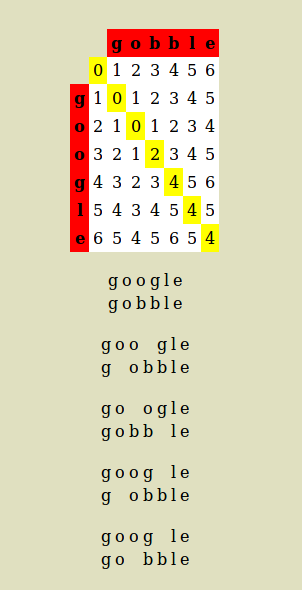
\includegraphics[width=0.8\textwidth]{levenshteindemo.png}
\end{frame}
